In diesem Abschnitt werden die Metriken an einem Besipiel demonstriert. Als Beispiel dient ein sehr einfacher BPEL-Prozess zur Verarbeitung von Bestellungen (Abbildung \ref{fig:Bespielprozess}).
\begin{figure}[htbp]
	\centering
		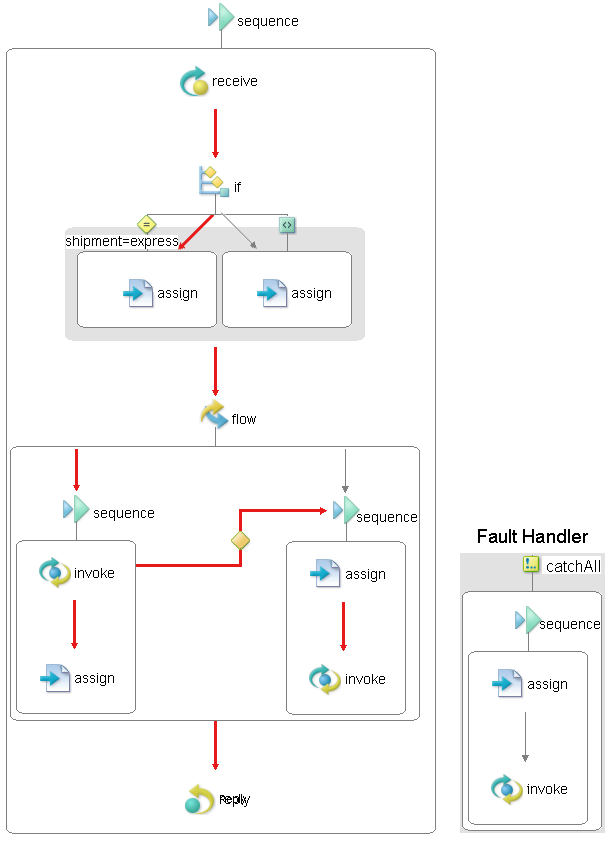
\includegraphics[width=0.45\textwidth]{bilder/Beispiel.png}
		\caption{Bespielprozess}
	\label{fig:Bespielprozess}
\end{figure}

Abh�ngig vom Liefertyp (\textit{express} oder \textit{normal}) werden die Bestellungsdaten unterschiedlich verarbeitet. Wenn der Kunde einen besonderen Status (VIP) hat, was mit dem \textit{Customer Identification}-Service festgestellt wird, dann wir der Kunde und sein Handelsvertreter �ber die Bestellung benachrichtigt.
Das wird mit Hilfe des Synchronisationslinks \textit{link\_1} modelliert, der eine explizite \textit{transition condition} aufweist: \textit{customerType='VIP'}.

Der Prozess bekommt in einem Testfall eine Bestellung eines \textit{VIP}-Kunden mit folgenden Daten:
\begin{verbatim}
<order>
    <shipment>express</shipment>
    <customerId>12345</customerId>
    <productId>46298</productId>
</order>
\end{verbatim}

Es ist nur wichtig zu wissen, dass der Kunde den VIP-Status hat. Bei der Bearbeitung der Daten wird der mit roten Pfeilen markierte Pfad durchlaufen.
Mit der Erweiterung des BPELUnit Frameworks kann die Testabdeckung ermittelt werden. Der Befehlszeilen-Client liefert die Testabdeckung im XML-Format: